\section{\texttt{shiny}}

%----------------------------------------------------------------------

\subsection*{Descrição}

\begin{frame}

  \texttt{shiny} torna incrivelmente fácil construir aplicações web
  interativas com o R. Ligação entre \emph{inputs} e \emph{outputs} que
  são reativos e um conjunto extenso de \emph{widgets} permitem
  construir interfaces atraentes, responsivas e poderosas para a web com
  esforço mínimo.

  \begin{itemize}
  \item Autores: Winston Chang, Joe Cheng, JJ Allaire, Yihui Xie,
    Jonathan McPherson, e muitos contribuidores
  \item Lançamento: 01-Dec-2012
  \item Versão: 0.12.1
  \item URL:
    \url{http://cran.r-project.org/web/packages/shiny/index.html},
    \url{http://shiny.rstudio.com/}
  \end{itemize}

\end{frame}

%----------------------------------------------------------------------

\subsection*{Como usar}

\begin{frame}
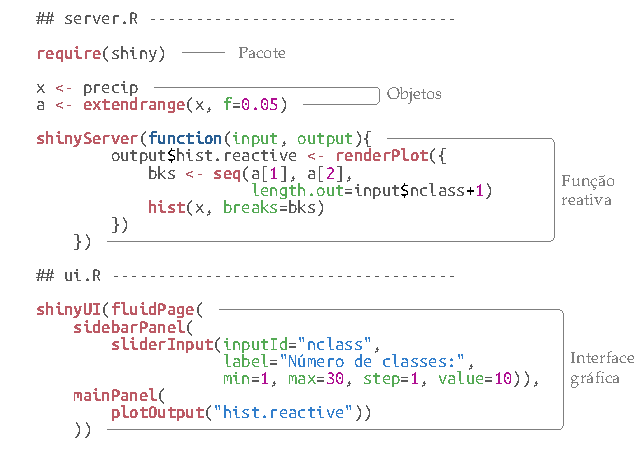
\includegraphics[scale=0.9]{./tikz/hist_slider_shiny-1.pdf}
\end{frame}

\begin{frame}
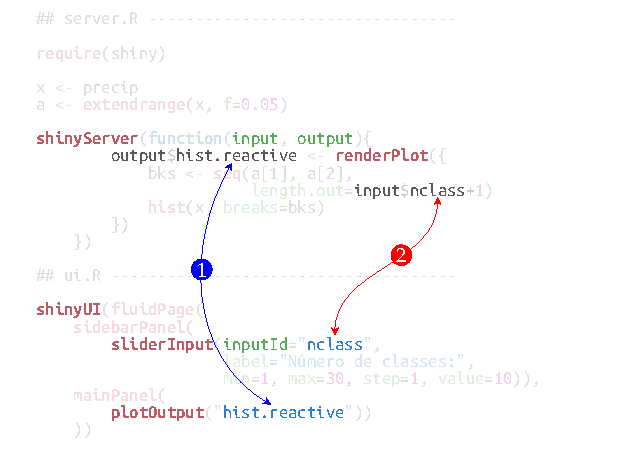
\includegraphics[scale=0.9]{./tikz/hist_slider_shiny-2.pdf}
\end{frame}

%----------------------------------------------------------------------

\subsection*{Exemplos}

\begin{frame}
 Praticando:
  \begin{enumerate}
  \item
    \href{run:./R/shiny/shiny}{R Scripts shiny (sliderInput)}\\
    \href{run:./R/shiny/shiny2}{R Scripts shiny (radioButtons)}
  \item 
	\href{http://200.17.213.89:3838/iguir/list/}{Galeria shiny IGUIR}
  \end{enumerate}
\end{frame}

\begin{frame}
  Algumas aplicações em \texttt{shiny}:
  \begin{itemize}
  \item \href{http://shiny.rstudio.com/gallery/}{Galeria Shiny Oficial},
  \item \href{http://www.showmeshiny.com/}{Galeria Shiny},
  \item \href{http://www.stat.cmu.edu:3838/hseltman/LogReg/}{Logistic
      Regression Residual Analysis},
  \item
    \href{https://hseltman.shinyapps.io/QuantileNormal}{Investigation of
      Quantile-Normal Plots Through Simulation},
  \item
    \href{http://www.stat.cmu.edu:3838/hseltman/PrePost/}{Pre-test/Post-test
      Simulation},
  \item
    \href{http://www.stat.cmu.edu:3838/hseltman/TransferFunctions/}{Explore
      Transfer Functions},
  \item
    \href{http://nbcgib.uesc.br/lec/avale-es/amb-virtual/inferencia/anava}{Fundamentos
      da análise de variância},
  \item
    \href{http://nbcgib.uesc.br/lec/avale-es/amb-virtual/probabilidade/con-frequentista}{Conceito
      frequentista de probabilidade}.
  \end{itemize}

\end{frame}
